\documentclass[a4paper]{article}

\usepackage[T1]{fontenc}
\usepackage[utf8]{inputenc}
\usepackage[english]{babel}
\usepackage{csquotes}
\usepackage{listings}
\usepackage{multicol}
\lstset{language=c,frame=single,captionpos=b}
\usepackage{hyperref}
\usepackage{amsmath}
\usepackage[backend=biber, sorting=none,maxbibnames=40]{biblatex}
\renewbibmacro{in:}{}
\addbibresource{ref.bib}
\usepackage{graphicx}
\usepackage{placeins}
\usepackage[margin=2.5cm]{geometry}
\usepackage{subcaption}
\usepackage[affil-it]{authblk}
\usepackage{color}
\usepackage{amssymb,amsmath}
\usepackage{subfloat}
\usepackage{float}

\begin{document}
\title{GPU Assignment: Image processing}
\author{Stefano Sandonà}
\affil{Vrije Universiteit Amsterdam, Holland}
\date{}
		
\maketitle

\section{GPUs: NVIDIA GTX480}
\label{sec:nvidia}
The aim of this assignement was to learn how to use many-core accelerators, GPUs in this particular case, to parallelize data-intensive code. All the implementations were written for the \textbf{NVIDIA GTX480}, using CUDA, a parallel computing platform and programming model invented by NVIDIA. Programming with CUDA, there is a straightforward mapping onto hardware, for this reason it is necessary to study the available HW before start developing an application. The main characteristics and the limits of the given accelerator, are showed in Table \ref{table:t1}.

\begin{table}[ht]
\centering
\caption{NVIDIA GTX480 Specifications}
\label{table:t1}
\begin{tabular}{l|l}
Microarchitecture & Fermi \\ \hline
Compute capability (version) & 2.0 \\ \hline
Maximum dimensionality of grid of thread blocks & 3 \\ \hline
Maximum x-dimension of a grid of thread blocks & 65535 \\ \hline
Maximum y-, or z-dimension of a grid of thread blocks & 65535 \\ \hline
Maximum dimensionality of thread block & 3 \\ \hline
Maximum x- or y-dimension of a block & 1024 \\ \hline
Maximum number of threads per block & 1024 \\ \hline
Cores per SM (warp size) & 32 \\ \hline
SM & 15 \\ \hline
Cores & 480 (32 * 15) \\ \hline
Maximum number of resident blocks per multiprocessor & 8 \\ \hline
Maximum number of resident warps per multiprocessor & 48 \\ \hline
Maximum number of resident threads per multiprocessor & 1536 (48 * 32) \\ \hline
Number of 32-bit registers per multiprocessor & 32K \\ \hline
Maximum amount of shared memory per multiprocessor & 48K
\end{tabular}
\end{table}

\section{CImg}
\label{sec:cimg}
The image processing library used in this project was CImg, a small, modern and open-source toolkit developed for C++. CImg implements the RGB color model, an additive color model in which red, green, and blue light are added together in various ways to reproduce a broad array of colors. Each colored image of size \textit{N x M} is composed by three parts (R,G,B) of the same size, so that \textit{N x M x 3} values are necessary to define an image. The Figure \ref{fig:rgb} shows an example of image composition.

\begin{figure}[ht]
    \centering
    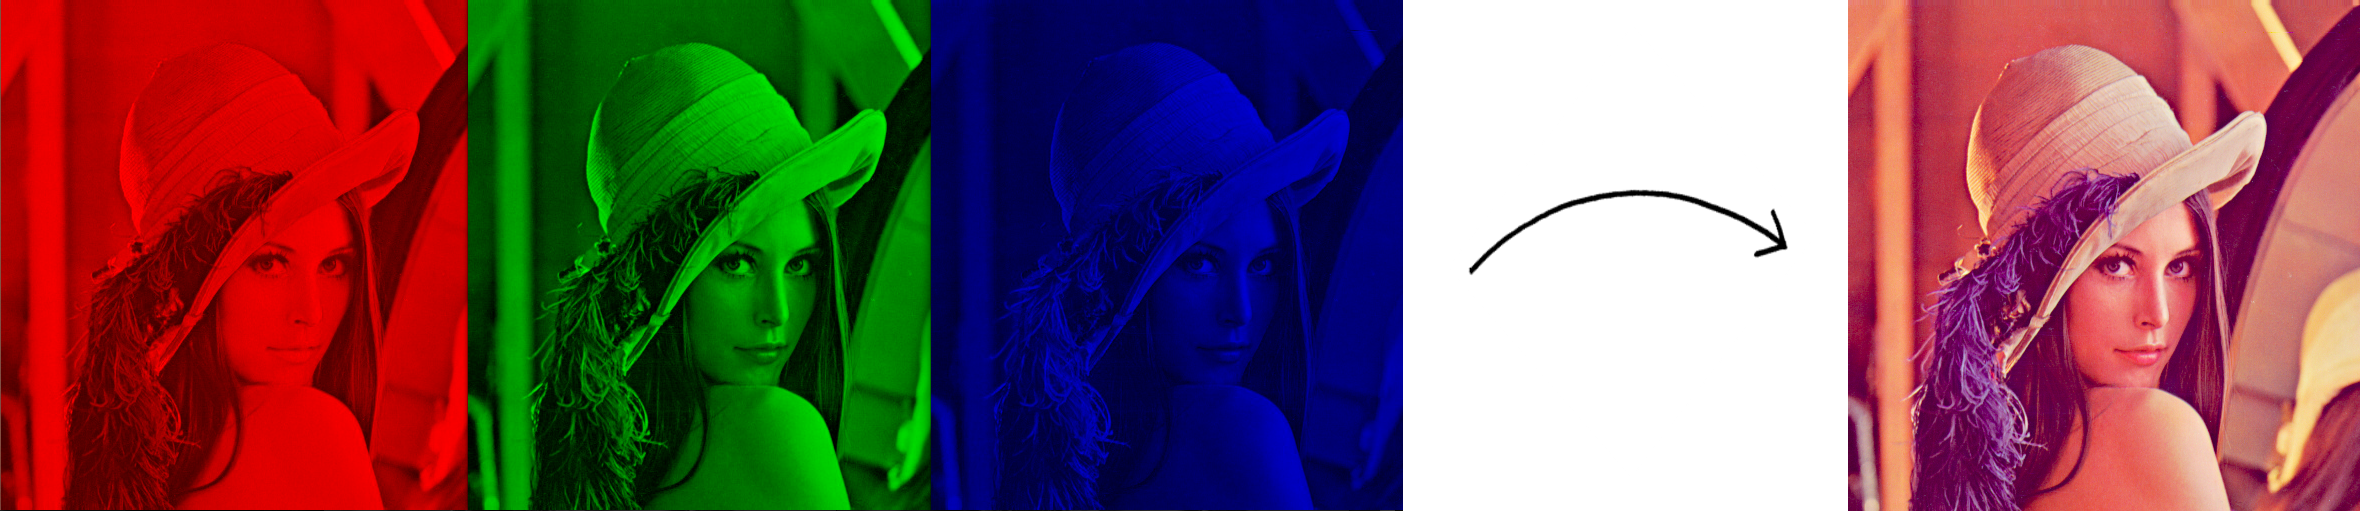
\includegraphics[width=0.7\linewidth]{rgb}
    \caption{RGB model}
    \label{fig:rgb}
\end{figure}
\FloatBarrier

\section{The processing flow}
\label{sec:cpf}
Using CUDA there are two parts of the code: the device code, or GPU code, or Kernel, that is a sequential program write for one thread and execute for all and the HOST code, or CPU code, that is used to instantiate the grid, run the kernel, manage the memory. Figure \ref{fig:flow} shows the processing flow of a CUDA application. In the particular case of image processig, everything starts from the CPU, that store the image from a file into a local buffer, allocates IN and OUT buffers on the GPU (\textit{cudaMalloc}) and copy the image into the GPU's IN buffer (\textit{cudaMemCpy}). After that, the CPU launches the GPU kernel with a defined grid configuration (\textit{kernel\_function <<gridDim, blockDim>>(params)}), that is executed by the GPU following the SIMT (Single Instruction, Multiple Threads) NVIDIA model. The threads are executed in parallel in each core, and they read the assigned part of IN data and generates the assigned part of OUT data. At the end, the results are copied out back to the CPU (\textit{cudaMemCpy}) and the image is written to a file by the CPU.

\begin{figure}[ht]
    \centering
    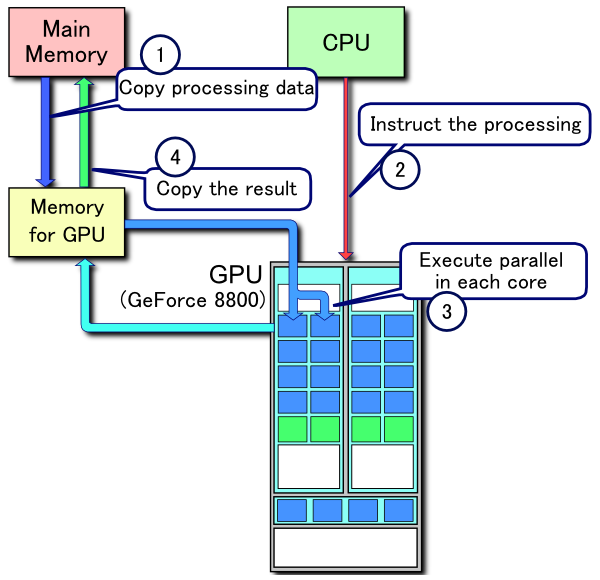
\includegraphics[width=0.5\linewidth]{flow}
    \caption{CUDA processing flow}
    \label{fig:flow}
\end{figure}
\FloatBarrier

\section{Algorithm 1: Grayscale Conversion and Darkening}
\label{sec:gcd}

\section{Algorithm 2: Histogram Computation}
\label{sec:hc}

\section{Algorithm 3: Smoothing}
\label{sec:smoo}


\printbibliography 

\end{document}

			 	 